\documentclass[12pt]{article}
% Full article preamble (duplicated, no common file)
\usepackage{fontspec}
\usepackage[a4paper,margin=2.5cm,includefoot]{geometry}
\usepackage{polyglossia}
\usepackage{amsmath}
\usepackage{amssymb}
\usepackage{xcolor}
\usepackage{fancyhdr}
\usepackage{graphicx}
\usepackage{listings}
\usepackage[most]{tcolorbox}
\usepackage{pifont}
\usepackage{enumitem}
\usepackage{titlesec}
\usepackage[bottom]{footmisc}
\usepackage{titling}
\usepackage{minted}
\usepackage{etoolbox}
\usepackage{array}
\usepackage{extsizes}

\newfontfamily\emoji{Segoe UI Emoji}

\pagestyle{fancy}

\setmainlanguage[numerals=western]{arabic}
\setotherlanguage{english}
\newfontfamily\arabicfont[Script=Arabic]{Amiri}
\newfontfamily\arabicfonttt[Script=Arabic]{Courier New}

\lstset{
  language=[Sharp]C,
  numbers=left,
  stepnumber=1,
  numbersep=8pt,
  frame=single,
  basicstyle=\ttfamily\small,
  keywordstyle=\color{blue},
  stringstyle=\color{red},
  commentstyle=\color{green!50!black}
}

\newif\ifdetailed
\ifdefined\setdetailed
  \setdetailed
\fi

\newif\ifwithsols
\ifdefined\setwithsols
  \setwithsols
\fi

% unified tcolorboxes for articles
\tcbset{colback=white, colframe=black, fonttitle=\bfseries, boxrule=0.8pt}
\newtcolorbox{boxDef}[1][]{colback=blue!5!white,colframe=blue!75!black,
  title={{\emoji📘} تعريف\ifx\\#1\\\else ~#1\fi :}}
\newtcolorbox{boxExercise}[1][]{colback=cyan!5!white,colframe=cyan!70!black,
  title={{\emoji🧩} تمرين\ifx\\#1\\\else ~#1\fi :}}
\newtcolorbox{boxExample}[1][]{colback=yellow!5!white,colframe=orange!90!black,
  title={{\emoji📝} مثال\ifx\\#1\\\else ~#1\fi :}}
\newtcolorbox{boxNote}[1][]{colback=gray!10!white,colframe=black,
  title={{\emoji✨} ملاحظة\ifx\\#1\\\else ~#1\fi :}}
\newtcolorbox{boxAttention}[1][]{colback=magenta!10!white,colframe=magenta!80!black,
  title={{\emoji🔔} تنبيه\ifx\\#1\\\else ~#1\fi :}}
\newtcolorbox{boxWarning}[1][]{colback=red!5!white,colframe=red!75!black,
  title={{\emoji⚡} ملاحظة هامة\ifx\\#1\\\else ~#1\fi :}}
\newtcolorbox{boxSolution}[1][]{colback=green!5!white,colframe=green!60!black,
  title={{\emoji✅} حل\ifx\\#1\\\else ~#1\fi :}}
\newtcolorbox{boxSymbol}[1][]{colback=purple!5!white,colframe=purple!70!black,
  title={{\emoji🔣} رمز\ifx\\#1\\\else ~#1\fi :}}

\tcbset{simplecode/.style={ colback=gray!5, colframe=black!50, boxrule=0.4pt, arc=2pt, left=4pt,right=4pt,top=4pt,bottom=4pt}}
\newenvironment{boxCode}{\begin{tcolorbox}[simplecode]}{\end{tcolorbox}}

\newcolumntype{C}[1]{>{\centering\arraybackslash}p{#1}}

% redefine spaces after titles
\makeatletter
\renewcommand{\@maketitle}{%
  \begin{center}
    {\huge \bfseries \@title \par}%
    \vskip 0.2em % space between title and author
    {\large \@author \par}%
    % \vskip 0.2em % space between author and date
    % {\normalsize \@date \par}%
  \end{center}
}
\makeatother

\fancyhf{} % clear default
\fancypagestyle{plain}{
  \fancyhf{}
  \fancyhead[L]{مدرسة التسامح الشاملة}
  % \fancyhead[L]{
\includegraphics[height=1cm]{../../../images/logoTasamoh.png}}
  \fancyhead[R]{الأستاذ محمود اغبارية}
  \fancyfoot[C]{\thepage}
}

\fancyhead[L]{مدرسة التسامح الشاملة}
\fancyhead[R]{الأستاذ محمود اغبارية}
\fancyfoot[C]{\thepage}
% \date{\today}

\setcounter{tocdepth}{3} % only section subsection and subsubsection in TOC


% ----------------------


% \begin{document}

% \maketitle

% % \clearpage  % start TOC on a new page
% % \renewcommand{\contentsname}{جدول المحتويات}
% % \tableofcontents
% % \clearpage

% \part*{part 1} % the * prevents numbering
% \section*{مقدمة}
% \subsection*{مثال رياضي}
% \subsubsection*{مثال فرعي}
% \paragraph*{ paragraph 1}
% \subparagraph*{sub paragraph 1}

% \ifdetailed
% \begin{english}
% \begin{minted}{csharp}
% // C# Example
% \end{minted}
% \end{english}
% \fi

% OLD WAY
% \ifdetailed
% \begin{english}
% \begin{lstlisting}
% // C# Example
% \end{lstlisting}
% \end{english}
% \fi

% % 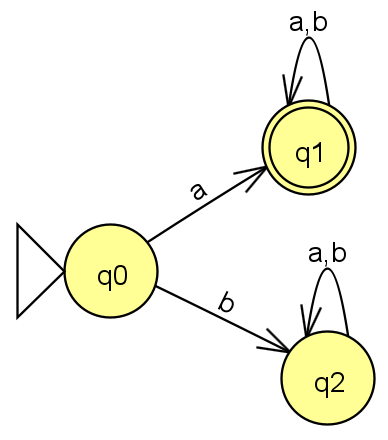
\includegraphics[width=0.2\textwidth]{../../../images/DFAs/ex1_q1.png}



% \vspace{3cm}
% \begin{flushleft}
% أرجو لكم وقتًا ممتعًا.

% الأستاذ محمود اغبارية.
% \end{flushleft}


% \end{document}


\title{ورقة تمرن 4 للصف العاشر 10 $\mathtt{if\ Statement}$}

\begin{document}

\maketitle
\thispagestyle{fancy}

\section{تمارين على الجمل الشريطة البسيطة}


\ifdetailed
\begin{enumerate}[itemsep=3em]
\else
\begin{enumerate}
\fi

\item
اكتب برنامجًا يستقبل من المستخدم درجة حرارة، ويطبع له "\textbf{الجو حار}" إذا كانت درجة الحرارة أكثر من 30 درجة.
\ifdetailed
\begin{example}[1]
\begin{english}
\begin{lstlisting}
Enter temperature:
35
It's hot
\end{lstlisting}
\end{english}
\end{example}
\begin{example}[2]
\begin{english}
\begin{lstlisting}
Enter temperature:
25
\end{lstlisting}
\end{english}
\end{example}

\ifwithsols
\begin{solution}
\begin{english}
\begin{lstlisting}
private static void Main(string[] args)
{
    Console.WriteLine("Enter temperature:");
    int temperature = int.Parse(Console.ReadLine());
    if (temperature > 30)
    {
        Console.WriteLine("It's hot");
    }
}
\end{lstlisting}
\end{english}
\end{solution}
\clearpage
\fi
\fi

\item
اكتب برنامجًا يستقبل من المستخدم رقمين، ويطبع له "\textbf{الرقم الأول أكبر}" إذا كان الرقم الأول أكبر من الثاني، و"\textbf{الرقم الثاني أكبر}" إذا كان الرقم الثاني أكبر من الأول.
\ifdetailed
\begin{example}[1]
\begin{english}
\begin{lstlisting}
Enter first number:
15
Enter second number:
10
The first number is larger
\end{lstlisting}
\end{english}
\end{example}
\begin{example}[2]
\begin{english}
\begin{lstlisting}
Enter first number:
5
Enter second number:
12
The second number is larger
\end{lstlisting}
\end{english}
\end{example}

\ifwithsols
\begin{solution}
\begin{english}
\begin{lstlisting}
private static void Main(string[] args)
{
    Console.WriteLine("Enter first number:");
    int num1 = int.Parse(Console.ReadLine());
    Console.WriteLine("Enter second number:");
    int num2 = int.Parse(Console.ReadLine());
    if (num1 > num2)
    {
        Console.WriteLine("The first number is larger");
    }
    else
    {
        Console.WriteLine("The second number is larger");
    }
}
\end{lstlisting}
\end{english}
\end{solution}
\clearpage
\fi
\fi

\item
اكتب برنامجًا يستقبل من المستخدم رقمين، ويطبع له "\textbf{لهما نفس الإشارة}" إذا كان كلاهما موجبَين أو كلاهما سالبين، و"\textbf{إشارتان مختلفتان}" إذا كان أحدهما موجبًا والآخر سالبًا.
(افترض أنّ الرقمين ليسا صفرًا.)
\ifdetailed
\begin{example}[1]
\begin{english}
\begin{lstlisting}
Enter first number:
5
Enter second number:
-3
Different signs
\end{lstlisting}
\end{english}
\end{example}
\begin{example}[2]
\begin{english}
\begin{lstlisting}
Enter first number:
-4
Enter second number:
-7
Same sign
\end{lstlisting}
\end{english}
\end{example}

\ifwithsols
\begin{solution}
\begin{english}
\begin{lstlisting}
private static void Main(string[] args)
{
    Console.WriteLine("Enter first number:");
    int num1 = int.Parse(Console.ReadLine());
    Console.WriteLine("Enter second number:");
    int num2 = int.Parse(Console.ReadLine());

    int product = num1 * num2;
    if (product > 0)
    {
        Console.WriteLine("Same sign");
    }
    else
    {
        Console.WriteLine("Different signs");
    }
}
\end{lstlisting}
\end{english}
\end{solution}
\clearpage
\fi
\fi

\item
اكتب برنامجًا يستقبل من المستخدم علامة طالب، ويطبع له التقدير المناسب حسب العلامة:
\begin{itemize}
\item \texttt{A+} إذا كانت العلامة 95 أو أكثر
\item \texttt{A} إذا كانت العلامة 90-94
\item \texttt{A-} إذا كانت العلامة 85-89
\item \texttt{B+} إذا كانت العلامة 80-84
\item \texttt{B} إذا كانت العلامة 75-79
\item \texttt{B-} إذا كانت العلامة 70-74
\item \texttt{C} إذا كانت العلامة أقل من 70
\end{itemize}
\ifdetailed
\begin{example}[1]
\begin{english}
\begin{lstlisting}
Enter your grade:
97
A+
\end{lstlisting}
\end{english}
\end{example}
\begin{example}[2]
\begin{english}
\begin{lstlisting}
Enter your grade:
82
B+
\end{lstlisting}
\end{english}
\end{example}
\begin{example}[3]
\begin{english}
\begin{lstlisting}
Enter your grade:
65
C
\end{lstlisting}
\end{english}
\end{example}

\ifwithsols
\begin{solution}
\begin{english}
\begin{lstlisting}
private static void Main(string[] args)
{
    Console.WriteLine("Enter your grade:");
    int grade = int.Parse(Console.ReadLine());
    if (grade >= 95)
    {
        Console.WriteLine("A+");
    }
    else if (grade >= 90)
    {
        Console.WriteLine("A");
    }
    else if (grade >= 85)
    {
        Console.WriteLine("A-");
    }
    else if (grade >= 80)
    {
        Console.WriteLine("B+");
    }
    else if (grade >= 75)
    {
        Console.WriteLine("B");
    }
    else if (grade >= 70)
    {
        Console.WriteLine("B-");
    }
    else
    {
        Console.WriteLine("C");
    }
}
\end{lstlisting}
\end{english}
\end{solution}
\clearpage
\fi
\fi

\end{enumerate}

\section{جمل شرطية متداخلة}

\ifdetailed
\begin{enumerate}[itemsep=3em]
\else
\begin{enumerate}
\fi

\item
اكتب برنامجًا يستقبل من المستخدم نوع الحيوان \texttt{C} للقط، \texttt{D} للكلب وعمره بالأشهر، ويطبع له رسالة مناسبة:
\begin{itemize}
\item إذا كان قط وعمره 12 شهر أو أكثر: "\textbf{قط بالغ}"
\item إذا كان قط وعمره أقل من 12 شهر: "\textbf{قط صغير}"
\item إذا كان كلب وعمره 12 شهر أو أكثر: "\textbf{كلب بالغ}"
\item إذا كان كلب وعمره أقل من 12 شهر: "\textbf{كلب صغير}"
\end{itemize}
\ifdetailed
\begin{example}[1]
\begin{english}
\begin{lstlisting}
Enter animal type (C=Cat, D=Dog):
C
Enter age in months:
18
Adult cat
\end{lstlisting}
\end{english}
\end{example}
\begin{example}[2]
\begin{english}
\begin{lstlisting}
Enter animal type (C=Cat, D=Dog):
D
Enter age in months:
8
Young dog
\end{lstlisting}
\end{english}
\end{example}

\ifwithsols
\begin{solution}
\begin{english}
\begin{lstlisting}
private static void Main(string[] args)
{
    Console.WriteLine("Enter animal type (C=Cat, D=Dog):");
    char animalType = char.Parse(Console.ReadLine());
    Console.WriteLine("Enter age in months:");
    int age = int.Parse(Console.ReadLine());

    if (animalType == 'C')
    {
        if (age >= 12)
        {
            Console.WriteLine("Adult cat");
        }
        else
        {
            Console.WriteLine("Young cat");
        }
    }
    else
    {
        if (age >= 12)
        {
            Console.WriteLine("Adult dog");
        }
        else
        {
            Console.WriteLine("Young dog");
        }
    }
}
\end{lstlisting}
\end{english}
\end{solution}
\clearpage
\fi
\fi

\item
اكتب برنامجًا يستقبل من المستخدم درجة حرارة وموسم السنة (1 للشتاء، 2 للصيف)، ويطبع له رسالة مناسبة:
\begin{itemize}
\item متوسط درجة الحرارة في الشتاء: 15 درجة
\item متوسط درجة الحرارة في الصيف: 30 درجة
\item إذا كانت درجة الحرارة أعلى من المتوسط: "\textbf{درجة الحرارة أعلى من المعدّل في [اسم الفصل]}"
\item إذا كانت درجة الحرارة أقل من أو تساوي المتوسط: "\textbf{درجة الحرارة أقل من أو تساوي المعدّل في [اسم الفصل]}"
\end{itemize}
\ifdetailed
\begin{example}[1]
\begin{english}
\begin{lstlisting}
Enter temperature:
20
Enter season (1=Winter, 2=Summer):
1
The temperature is higher than the average in Winter
\end{lstlisting}
\end{english}
\end{example}
\begin{example}[2]
\begin{english}
\begin{lstlisting}
Enter temperature:
25
Enter season (1=Winter, 2=Summer):
2
The temperature is lower than or equal to the average in Summer
\end{lstlisting}
\end{english}
\end{example}

\ifwithsols
\begin{solution}
\begin{english}
\begin{lstlisting}
private static void Main(string[] args)
{
    Console.WriteLine("Enter temperature:");
    int temperature = int.Parse(Console.ReadLine());
    Console.WriteLine("Enter season (1=Winter, 2=Summer):");
    int season = int.Parse(Console.ReadLine());

    if (season == 1)
    {
        if (temperature > 15)
        {
            Console.WriteLine("The temperature is higher than the average in Winter");
        }
        else
        {
            Console.WriteLine("The temperature is lower than or equal to the average in Winter");
        }
    }
    else
    {
        if (temperature > 30)
        {
            Console.WriteLine("The temperature is higher than the average in Summer");
        }
        else
        {
            Console.WriteLine("The temperature is lower than or equal to the average in Summer");
        }
    }
}
\end{lstlisting}
\end{english}
\end{solution}
\clearpage
\fi
\fi

\item
اكتب برنامجًا يستقبل من المستخدم نوع الحساب المصرفي (\texttt{S} لحساب التوفير، \texttt{C} للحساب الجاري) والرصيد الحالي ومبلغ السحب، ويطبع له رسالة مناسبة:
\begin{itemize}
\item إذا كان حساب توفير ورصيده 1000 أو أكثر ومبلغ السحب 500 أو أقل: "\textbf{سحب ناجح من حساب التوفير}"
\item إذا كان حساب توفير ورصيده 1000 أو أكثر ومبلغ السحب أكثر من 500: "\textbf{مبلغ السحب كبير جداً لحساب التوفير}"
\item إذا كان حساب توفير ورصيده أقل من 1000 ومبلغ السحب 200 أو أقل: "\textbf{سحب ناجح من حساب التوفير}"
\item إذا كان حساب توفير ورصيده أقل من 1000 ومبلغ السحب أكثر من 200: "\textbf{رصيد غير كافي في حساب التوفير}"
\item إذا كان حساب جاري ورصيده 500 أو أكثر ومبلغ السحب 1000 أو أقل: "\textbf{سحب ناجح من الحساب الجاري}"
\item إذا كان حساب جاري ورصيده 500 أو أكثر ومبلغ السحب أكثر من 1000: "\textbf{مبلغ السحب كبير جداً للحساب الجاري}"
\item إذا كان حساب جاري ورصيده أقل من 500 ومبلغ السحب 300 أو أقل: "\textbf{سحب ناجح من الحساب الجاري}"
\item إذا كان حساب جاري ورصيده أقل من 500 ومبلغ السحب أكثر من 300: "\textbf{رصيد غير كافي في الحساب الجاري}"
\end{itemize}
\ifdetailed
\begin{example}[1]
\begin{english}
\begin{lstlisting}
Enter account type (S=Savings, C=Current):
S
Enter current balance:
1500
Enter withdrawal amount:
300
Withdrawal successful from savings account
\end{lstlisting}
\end{english}
\end{example}
\begin{example}[2]
\begin{english}
\begin{lstlisting}
Enter account type (S=Savings, C=Current):
C
Enter current balance:
800
Enter withdrawal amount:
1200
Withdrawal amount too large for current account
\end{lstlisting}
\end{english}
\end{example}
\begin{example}[3]
\begin{english}
\begin{lstlisting}
Enter account type (S=Savings, C=Current):
S
Enter current balance:
800
Enter withdrawal amount:
250
Insufficient balance in savings account
\end{lstlisting}
\end{english}
\end{example}

\ifwithsols
\begin{solution}
\begin{english}
\begin{lstlisting}
private static void Main(string[] args)
{
    Console.WriteLine("Enter account type (S=Savings, C=Current):");
    char accountType = char.Parse(Console.ReadLine());
    Console.WriteLine("Enter current balance:");
    int balance = int.Parse(Console.ReadLine());
    Console.WriteLine("Enter withdrawal amount:");
    int withdrawal = int.Parse(Console.ReadLine());

    if (accountType == 'S')
    {
        if (balance >= 1000)
        {
            if (withdrawal <= 500)
            {
                Console.WriteLine("Withdrawal successful from savings account");
            }
            else
            {
                Console.WriteLine("Withdrawal amount too large for savings account");
            }
        }
        else
        {
            if (withdrawal <= 200)
            {
                Console.WriteLine("Withdrawal successful from savings account");
            }
            else
            {
                Console.WriteLine("Insufficient balance in savings account");
            }
        }
    }
    else
    {
        if (balance >= 500)
        {
            if (withdrawal <= 1000)
            {
                Console.WriteLine("Withdrawal successful from current account");
            }
            else
            {
                Console.WriteLine("Withdrawal amount too large for current account");
            }
        }
        else
        {
            if (withdrawal <= 300)
            {
                Console.WriteLine("Withdrawal successful from current account");
            }
            else
            {
                Console.WriteLine("Insufficient balance in current account");
            }
        }
    }
}
\end{lstlisting}
\end{english}
\end{solution}
\clearpage
\fi
\fi

\end{enumerate}

\section{جمل شرطية مع "وأيضًا"}

\ifdetailed
\begin{enumerate}[itemsep=3em]
\else
\begin{enumerate}
\fi

\item
اكتب برنامجًا يستقبل من المستخدم عمر شخص ودرجة حرارة، ويطبع له "\textbf{يمكنك الخروج}" إذا كان عمره 18 أو أكثر ودرجة الحرارة أقل من 35.
\ifdetailed
\begin{example}[1]
\begin{english}
\begin{lstlisting}
Enter your age:
20
Enter temperature:
30
You can go out
\end{lstlisting}
\end{english}
\end{example}
\begin{example}[2]
\begin{english}
\begin{lstlisting}
Enter your age:
16
Enter temperature:
30
\end{lstlisting}
\end{english}
\end{example}

\ifwithsols
\begin{solution}
\begin{english}
\begin{lstlisting}
private static void Main(string[] args)
{
    Console.WriteLine("Enter your age:");
    int age = int.Parse(Console.ReadLine());
    Console.WriteLine("Enter temperature:");
    int temperature = int.Parse(Console.ReadLine());

    if (age >= 18 && temperature < 35)
    {
        Console.WriteLine("You can go out");
    }
}
\end{lstlisting}
\end{english}
\end{solution}
\clearpage
\fi
\fi

\item
اكتب برنامجًا يستقبل من المستخدم رقمين، ويطبع له "\textbf{الرقمان موجبان}" إذا كان كلاهما أكبر من صفر.
\ifdetailed
\begin{example}[1]
\begin{english}
\begin{lstlisting}
Enter first number:
5
Enter second number:
8
Both numbers are positive
\end{lstlisting}
\end{english}
\end{example}
\begin{example}[2]
\begin{english}
\begin{lstlisting}
Enter first number:
-3
Enter second number:
7
\end{lstlisting}
\end{english}
\end{example}

\ifwithsols
\begin{solution}
\begin{english}
\begin{lstlisting}
private static void Main(string[] args)
{
    Console.WriteLine("Enter first number:");
    int num1 = int.Parse(Console.ReadLine());
    Console.WriteLine("Enter second number:");
    int num2 = int.Parse(Console.ReadLine());

    if (num1 > 0 && num2 > 0)
    {
        Console.WriteLine("Both numbers are positive");
    }
}
\end{lstlisting}
\end{english}
\end{solution}
\clearpage
\fi
\fi

\item
اكتب برنامجًا يستقبل من المستخدم علامة طالب وعمره، ويطبع له "\textbf{طالب ممتاز}" إذا كانت علامته 90 أو أكثر وعمره 16 أو أكثر.
\ifdetailed
\begin{example}[1]
\begin{english}
\begin{lstlisting}
Enter your grade:
95
Enter your age:
18
Excellent student
\end{lstlisting}
\end{english}
\end{example}
\begin{example}[2]
\begin{english}
\begin{lstlisting}
Enter your grade:
85
Enter your age:
17
\end{lstlisting}
\end{english}
\end{example}

\ifwithsols
\begin{solution}
\begin{english}
\begin{lstlisting}
private static void Main(string[] args)
{
    Console.WriteLine("Enter your grade:");
    int grade = int.Parse(Console.ReadLine());
    Console.WriteLine("Enter your age:");
    int age = int.Parse(Console.ReadLine());

    if (grade >= 90 && age >= 16)
    {
        Console.WriteLine("Excellent student");
    }
}
\end{lstlisting}
\end{english}
\end{solution}
\clearpage
\fi
\fi

\end{enumerate}

\section{جمل شرطية مع "أو"}

\ifdetailed
\begin{enumerate}[itemsep=3em]
\else
\begin{enumerate}
\fi

\item
اكتب برنامجًا يستقبل من المستخدم درجة حرارة، ويطبع له "\textbf{الجو غير مناسب}" إذا كانت درجة الحرارة أقل من 10 أو أكثر من 40.
\ifdetailed
\begin{example}[1]
\begin{english}
\begin{lstlisting}
Enter temperature:
5
Weather is not suitable
\end{lstlisting}
\end{english}
\end{example}
\begin{example}[2]
\begin{english}
\begin{lstlisting}
Enter temperature:
25
\end{lstlisting}
\end{english}
\end{example}

\ifwithsols
\begin{solution}
\begin{english}
\begin{lstlisting}
private static void Main(string[] args)
{
    Console.WriteLine("Enter temperature:");
    int temperature = int.Parse(Console.ReadLine());

    if (temperature < 10 || temperature > 40)
    {
        Console.WriteLine("Weather is not suitable");
    }
}
\end{lstlisting}
\end{english}
\end{solution}
\clearpage
\fi
\fi

\item
اكتب برنامجًا يستقبل من المستخدم رقم، ويطبع له "\textbf{الرقم صحيح}" إذا كان الرقم 1 أو 2 أو 3.
\ifdetailed
\begin{example}[1]
\begin{english}
\begin{lstlisting}
Enter a number:
2
The number is valid
\end{lstlisting}
\end{english}
\end{example}
\begin{example}[2]
\begin{english}
\begin{lstlisting}
Enter a number:
5
\end{lstlisting}
\end{english}
\end{example}

\ifwithsols
\begin{solution}
\begin{english}
\begin{lstlisting}
private static void Main(string[] args)
{
    Console.WriteLine("Enter a number:");
    int number = int.Parse(Console.ReadLine());

    if (number == 1 || number == 2 || number == 3)
    {
        Console.WriteLine("The number is valid");
    }
}
\end{lstlisting}
\end{english}
\end{solution}
\clearpage
\fi
\fi

\item
اكتب برنامجًا يستقبل من المستخدم نوع اليوم (1 للعمل، 2 للعطلة) ودرجة الحرارة، ويطبع له "\textbf{يوم ممتع}" إذا كان يوم عطلة أو درجة الحرارة مثالية (20-25).
\ifdetailed
\begin{example}[1]
\begin{english}
\begin{lstlisting}
Enter day type (1=Work, 2=Holiday):
2
Enter temperature:
30
Enjoyable day
\end{lstlisting}
\end{english}
\end{example}
\begin{example}[2]
\begin{english}
\begin{lstlisting}
Enter day type (1=Work, 2=Holiday):
1
Enter temperature:
22
Enjoyable day
\end{lstlisting}
\end{english}
\end{example}

\ifwithsols
\begin{solution}
\begin{english}
\begin{lstlisting}
private static void Main(string[] args)
{
    Console.WriteLine("Enter day type (1=Work, 2=Holiday):");
    int dayType = int.Parse(Console.ReadLine());
    Console.WriteLine("Enter temperature:");
    int temperature = int.Parse(Console.ReadLine());

    if (dayType == 2 || (temperature >= 20 && temperature <= 25))
    {
        Console.WriteLine("Enjoyable day");
    }
}
\end{lstlisting}
\end{english}
\end{solution}
\clearpage
\fi
\fi

\end{enumerate}

\section{جمل شرطية مع "وأيضًا" و "أو"}

\ifdetailed
\begin{enumerate}[itemsep=3em]
\else
\begin{enumerate}
\fi

\item
اكتب برنامجًا يستقبل من المستخدم نوع الحساب (\texttt{S} للتوفير، \texttt{C} للجاري) والرصيد ومبلغ السحب، ويطبع له "\textbf{سحب مسموح}" إذا كان حساب توفير ورصيده 1000 أو أكثر، أو حساب جاري ورصيده 500 أو أكثر، ومبلغ السحب 200 أو أقل.
\ifdetailed
\begin{example}[1]
\begin{english}
\begin{lstlisting}
Enter account type (S=Savings, C=Current):
S
Enter balance:
1500
Enter withdrawal amount:
150
Withdrawal allowed
\end{lstlisting}
\end{english}
\end{example}
\begin{example}[2]
\begin{english}
\begin{lstlisting}
Enter account type (S=Savings, C=Current):
C
Enter balance:
300
Enter withdrawal amount:
100
\end{lstlisting}
\end{english}
\end{example}

\ifwithsols
\begin{solution}
\begin{english}
\begin{lstlisting}
private static void Main(string[] args)
{
    Console.WriteLine("Enter account type (S=Savings, C=Current):");
    char accountType = char.Parse(Console.ReadLine());
    Console.WriteLine("Enter balance:");
    int balance = int.Parse(Console.ReadLine());
    Console.WriteLine("Enter withdrawal amount:");
    int withdrawal = int.Parse(Console.ReadLine());

    if ((accountType == 'S' && balance >= 1000) || (accountType == 'C' && balance >= 500))
    {
        if (withdrawal <= 200)
        {
            Console.WriteLine("Withdrawal allowed");
        }
    }
}
\end{lstlisting}
\end{english}
\end{solution}
\clearpage
\fi
\fi

\item
اكتب برنامجًا يستقبل من المستخدم العمر والجنس (\texttt{M} للذكر، \texttt{F} للأنثى) ودرجة الحرارة، ويطبع له "\textbf{يمكنك السباحة}" إذا كان ذكر وعمره 12 أو أكثر، أو أنثى وعمرها 10 أو أكثر، ودرجة الحرارة 25 أو أكثر.
\ifdetailed
\begin{example}[1]
\begin{english}
\begin{lstlisting}
Enter age:
15
Enter gender (M/F):
M
Enter temperature:
28
You can swim
\end{lstlisting}
\end{english}
\end{example}
\begin{example}[2]
\begin{english}
\begin{lstlisting}
Enter age:
8
Enter gender (M/F):
F
Enter temperature:
30
\end{lstlisting}
\end{english}
\end{example}

\ifwithsols
\begin{solution}
\begin{english}
\begin{lstlisting}
private static void Main(string[] args)
{
    Console.WriteLine("Enter age:");
    int age = int.Parse(Console.ReadLine());
    Console.WriteLine("Enter gender (M/F):");
    char gender = char.Parse(Console.ReadLine());
    Console.WriteLine("Enter temperature:");
    int temperature = int.Parse(Console.ReadLine());

    if ((gender == 'M' && age >= 12) || (gender == 'F' && age >= 10))
    {
        if (temperature >= 25)
        {
            Console.WriteLine("You can swim");
        }
    }
}
\end{lstlisting}
\end{english}
\end{solution}
\clearpage
\fi
\fi

\item
اكتب برنامجًا يستقبل من المستخدم نوع الطالب (\texttt{S} للطالب، \texttt{T} للمعلم) والعلامة والسنوات من الخبرة، ويطبع له "\textbf{مؤهل للترقية}" إذا كان طالب وعلامته 85 أو أكثر، أو معلم وعلامته 90 أو أكثر وسنوات الخبرة 3 أو أكثر.
\ifdetailed
\begin{example}[1]
\begin{english}
\begin{lstlisting}
Enter person type (S=Student, T=Teacher):
S
Enter grade:
90
Enter years of experience:
0
Eligible for promotion
\end{lstlisting}
\end{english}
\end{example}
\begin{example}[2]
\begin{english}
\begin{lstlisting}
Enter person type (S=Student, T=Teacher):
T
Enter grade:
95
Enter years of experience:
5
Eligible for promotion
\end{lstlisting}
\end{english}
\end{example}

\ifwithsols
\begin{solution}
\begin{english}
\begin{lstlisting}
private static void Main(string[] args)
{
    Console.WriteLine("Enter person type (S=Student, T=Teacher):");
    char personType = char.Parse(Console.ReadLine());
    Console.WriteLine("Enter grade:");
    int grade = int.Parse(Console.ReadLine());
    Console.WriteLine("Enter years of experience:");
    int experience = int.Parse(Console.ReadLine());

    if ((personType == 'S' && grade >= 85) || (personType == 'T' && grade >= 90 && experience >= 3))
    {
        Console.WriteLine("Eligible for promotion");
    }
}
\end{lstlisting}
\end{english}
\end{solution}
\clearpage
\fi
\fi

\end{enumerate}

\section{جمل شرطية مع نفي}

\ifdetailed
\begin{enumerate}[itemsep=3em]
\else
\begin{enumerate}
\fi

\item
اكتب برنامجًا يستقبل من المستخدم رقم، ويطبع له "\textbf{الرقم ليس صفر}" إذا كان الرقم لا يساوي صفر.
\ifdetailed
\begin{example}[1]
\begin{english}
\begin{lstlisting}
Enter a number:
5
The number is not zero
\end{lstlisting}
\end{english}
\end{example}
\begin{example}[2]
\begin{english}
\begin{lstlisting}
Enter a number:
0
\end{lstlisting}
\end{english}
\end{example}

\ifwithsols
\begin{solution}
\begin{english}
\begin{lstlisting}
private static void Main(string[] args)
{
    Console.WriteLine("Enter a number:");
    int number = int.Parse(Console.ReadLine());

    if (!(number == 0))
    {
        Console.WriteLine("The number is not zero");
    }
}
\end{lstlisting}
\end{english}
\end{solution}
\clearpage
\fi
\fi

\item
اكتب برنامجًا يستقبل من المستخدم درجة حرارة، ويطبع له "\textbf{الجو ليس بارد}" إذا كانت درجة الحرارة ليست أقل من 15.
\ifdetailed
\begin{example}[1]
\begin{english}
\begin{lstlisting}
Enter temperature:
20
Weather is not cold
\end{lstlisting}
\end{english}
\end{example}
\begin{example}[2]
\begin{english}
\begin{lstlisting}
Enter temperature:
10
\end{lstlisting}
\end{english}
\end{example}

\ifwithsols
\begin{solution}
\begin{english}
\begin{lstlisting}
private static void Main(string[] args)
{
    Console.WriteLine("Enter temperature:");
    int temperature = int.Parse(Console.ReadLine());

    if (!(temperature < 15))
    {
        Console.WriteLine("Weather is not cold");
    }
}
\end{lstlisting}
\end{english}
\end{solution}
\clearpage
\fi
\fi

\item
اكتب برنامجًا يستقبل من المستخدم رقمين، ويطبع له "\textbf{الرقمان غير متساويين}" إذا كان الرقم الأول لا يساوي الثاني.
\ifdetailed
\begin{example}[1]
\begin{english}
\begin{lstlisting}
Enter first number:
5
Enter second number:
8
The numbers are not equal
\end{lstlisting}
\end{english}
\end{example}
\begin{example}[2]
\begin{english}
\begin{lstlisting}
Enter first number:
7
Enter second number:
7
\end{lstlisting}
\end{english}
\end{example}

\ifwithsols
\begin{solution}
\begin{english}
\begin{lstlisting}
private static void Main(string[] args)
{
    Console.WriteLine("Enter first number:");
    int num1 = int.Parse(Console.ReadLine());
    Console.WriteLine("Enter second number:");
    int num2 = int.Parse(Console.ReadLine());

    if (!(num1 == num2))
    {
        Console.WriteLine("The numbers are not equal");
    }
}
\end{lstlisting}
\end{english}
\end{solution}
\clearpage
\fi
\fi

\end{enumerate}

\section{جمل شرطية مركبة من كل العمليات}

\ifdetailed
\begin{enumerate}[itemsep=3em]
\else
\begin{enumerate}
\fi

\item
اكتب برنامجًا يستقبل من المستخدم نوع الحساب (\texttt{S} للتوفير، \texttt{C} للجاري) والرصيد ومبلغ السحب، ويطبع له "\textbf{سحب مسموح}" إذا كان حساب توفير ورصيده 1000 أو أكثر ومبلغ السحب ليس أكثر من 500، أو حساب جاري ورصيده 500 أو أكثر ومبلغ السحب ليس أكثر من 1000.
\ifdetailed
\begin{example}[1]
\begin{english}
\begin{lstlisting}
Enter account type (S=Savings, C=Current):
S
Enter balance:
1500
Enter withdrawal amount:
300
Withdrawal allowed
\end{lstlisting}
\end{english}
\end{example}
\begin{example}[2]
\begin{english}
\begin{lstlisting}
Enter account type (S=Savings, C=Current):
C
Enter balance:
800
Enter withdrawal amount:
1200
\end{lstlisting}
\end{english}
\end{example}

\ifwithsols
\begin{solution}
\begin{english}
\begin{lstlisting}
private static void Main(string[] args)
{
    Console.WriteLine("Enter account type (S=Savings, C=Current):");
    char accountType = char.Parse(Console.ReadLine());
    Console.WriteLine("Enter balance:");
    int balance = int.Parse(Console.ReadLine());
    Console.WriteLine("Enter withdrawal amount:");
    int withdrawal = int.Parse(Console.ReadLine());

    if ((accountType == 'S' && balance >= 1000 && !(withdrawal > 500)) ||
        (accountType == 'C' && balance >= 500 && !(withdrawal > 1000)))
    {
        Console.WriteLine("Withdrawal allowed");
    }
}
\end{lstlisting}
\end{english}
\end{solution}
\clearpage
\fi
\fi

\item
اكتب برنامجًا يستقبل من المستخدم العمر والجنس (\texttt{M} للذكر، \texttt{F} للأنثى) ودرجة الحرارة، ويطبع له "\textbf{يمكنك المشاركة}" إذا كان ذكر وعمره 18 أو أكثر ودرجة الحرارة ليست أقل من 20، أو أنثى وعمرها 16 أو أكثر ودرجة الحرارة ليست أكثر من 35.
\ifdetailed
\begin{example}[1]
\begin{english}
\begin{lstlisting}
Enter age:
20
Enter gender (M/F):
M
Enter temperature:
25
You can participate
\end{lstlisting}
\end{english}
\end{example}
\begin{example}[2]
\begin{english}
\begin{lstlisting}
Enter age:
17
Enter gender (M/F):
F
Enter temperature:
30
You can participate
\end{lstlisting}
\end{english}
\end{example}

\ifwithsols
\begin{solution}
\begin{english}
\begin{lstlisting}
private static void Main(string[] args)
{
    Console.WriteLine("Enter age:");
    int age = int.Parse(Console.ReadLine());
    Console.WriteLine("Enter gender (M/F):");
    char gender = char.Parse(Console.ReadLine());
    Console.WriteLine("Enter temperature:");
    int temperature = int.Parse(Console.ReadLine());

    if ((gender == 'M' && age >= 18 && !(temperature < 20)) ||
        (gender == 'F' && age >= 16 && !(temperature > 35)))
    {
        Console.WriteLine("You can participate");
    }
}
\end{lstlisting}
\end{english}
\end{solution}
\clearpage
\fi
\fi

\item
اكتب برنامجًا يستقبل من المستخدم نوع الطالب (\texttt{S} للطالب، \texttt{T} للمعلم) والعلامة والسنوات من الخبرة، ويطبع له "\textbf{مؤهل للمنحة}" إذا كان طالب وعلامته 80 أو أكثر وليس أقل من 60، أو معلم وعلامته 85 أو أكثر وسنوات الخبرة 2 أو أكثر وليس أكثر من 10.
\ifdetailed
\begin{example}[1]
\begin{english}
\begin{lstlisting}
Enter person type (S=Student, T=Teacher):
S
Enter grade:
75
Enter years of experience:
0
Eligible for scholarship
\end{lstlisting}
\end{english}
\end{example}
\begin{example}[2]
\begin{english}
\begin{lstlisting}
Enter person type (S=Student, T=Teacher):
T
Enter grade:
90
Enter years of experience:
5
Eligible for scholarship
\end{lstlisting}
\end{english}
\end{example}

\ifwithsols
\begin{solution}
\begin{english}
\begin{lstlisting}
private static void Main(string[] args)
{
    Console.WriteLine("Enter person type (S=Student, T=Teacher):");
    char personType = char.Parse(Console.ReadLine());
    Console.WriteLine("Enter grade:");
    int grade = int.Parse(Console.ReadLine());
    Console.WriteLine("Enter years of experience:");
    int experience = int.Parse(Console.ReadLine());

    if ((personType == 'S' && grade >= 80 && !(grade < 60)) ||
        (personType == 'T' && grade >= 85 && experience >= 2 && !(experience > 10)))
    {
        Console.WriteLine("Eligible for scholarship");
    }
}
\end{lstlisting}
\end{english}
\end{solution}
\clearpage
\fi
\fi

\end{enumerate}

\vspace{3cm}
\begin{flushleft}
أرجو لكم وقتًا ممتعًا.

الأستاذ محمود اغبارية.
\end{flushleft}

\end{document}